% Báo cáo bài tập lớn RAG – biên dịch bằng pdfLaTeX (mặc định của Overleaf)
\documentclass[11pt,a4paper]{article}
\usepackage[utf8]{inputenc}
\usepackage[T5]{fontenc}
\usepackage[vietnamese]{babel}
\usepackage{lmodern}
\renewcommand{\rmdefault}{utm}   % Times (URW, hỗ trợ tiếng Việt), font chữ của chuẩn IEEE
\usepackage{microtype}     % giảm tràn lề
\emergencystretch=2em
\usepackage[a4paper,margin=2.3cm]{geometry}
\usepackage{graphicx}
\usepackage{booktabs}
\usepackage{tabularx}
\usepackage{multirow}
\usepackage{array}
\usepackage{float}
\usepackage{caption}
\usepackage{subcaption}
\usepackage{amsmath}
\usepackage{enumitem}
\usepackage{xcolor}
\usepackage{xurl}          % URL / đường dẫn dài được ngắt dòng
\usepackage{tikz}
\usetikzlibrary{positioning,arrows.meta,shapes.geometric}
\usepackage{cite}          % trích dẫn số theo IEEE: [1], [2]--[4]
\usepackage[colorlinks=true,linkcolor=blue!50!black,urlcolor=blue!60!black,citecolor=blue!50!black]{hyperref}

\graphicspath{{figures/}}
\setlist{nosep,leftmargin=*}
\addto\captionsvietnamese{\renewcommand{\refname}{Tài liệu tham khảo}}
\newcommand{\best}[1]{\textbf{#1}}
\newcommand{\file}[1]{\path{#1}}
\captionsetup{font=small}

% ======================= THÔNG TIN — SỬA Ở ĐÂY =======================
\newcommand{\hoten}{Đinh Thị Thu Thủy}
\newcommand{\mssv}{2570508}
\newcommand{\monhoc}{Mô hình ngôn ngữ lớn}
\newcommand{\nhom}{CH01}
\newcommand{\vaitro}{Học viên thực hiện}
\newcommand{\gvhd}{Quản Thành Thơ}
\newcommand{\khoa}{KHOA KHOA HỌC MÁY TÍNH}
\newcommand{\githublink}{https://github.com/dinhthithuthuyduphong-bot/LAB/tree/RAG-based-chatbot-system}
\newcommand{\videolink}{https://youtu.be/sOus4EisfnE}       % link video demo (YouTube)
% =====================================================================

\begin{document}
\begin{titlepage}
\centering
{\large ĐẠI HỌC QUỐC GIA THÀNH PHỐ HỒ CHÍ MINH\\[2pt]
TRƯỜNG ĐẠI HỌC BÁCH KHOA\\[2pt]
\textbf{\khoa}\par}
\vspace{1.2cm}
% Logo: đặt file figures/logo_hcmut.png (logo chính thức của trường) để logo tự hiện ở đây.
\IfFileExists{figures/logo_hcmut.png}{
\includegraphics[width=4.2cm]{logo_hcmut.png}\par\vspace{1.2cm}}{\vspace{3cm}}
{\Large\textbf{\MakeUppercase{\monhoc}}\par}
\vspace{0.8cm}
{\large BÁO CÁO BÀI TẬP LỚN\par}
\vspace{0.6cm}
\rule{\linewidth}{0.8pt}\par\vspace{0.3cm}
{\LARGE\textbf{CẢI TIẾN HỆ THỐNG RAG\\[4pt] CHO CHATBOT HỎI ĐÁP PHÁP LUẬT}\par}
\vspace{0.2cm}\rule{\linewidth}{0.8pt}\par
\vspace{1.8cm}
{\large
\begin{tabular}{@{}ll@{}}
Giảng viên hướng dẫn: & \gvhd \\[4pt]
\vaitro: & \hoten \\[4pt]
MSSV: & \mssv \\[4pt]
Nhóm: & \nhom \\
\end{tabular}\par}
\vfill
{\large TP. Hồ Chí Minh, tháng \the\month/\the\year\par}
\end{titlepage}

\begin{abstract}
Em cải tiến hệ thống RAG baseline (\texttt{vietnamese-sbert} + FAISS + \texttt{Qwen1.5-1.8B}) cho bài toán hỏi đáp pháp luật tiếng Việt.
Hệ thống cuối gồm: tiền xử lý văn bản và tách metadata, chia đoạn theo cấu trúc Chương/Điều, tìm kiếm kết hợp BM25 + dense (RRF),
xếp hạng lại bằng cross-encoder, mô hình \texttt{Qwen2.5-3B-Instruct} và prompt theo mẫu câu trả lời pháp lý kèm một ví dụ few-shot.
Trên cùng \textbf{200 cặp hỏi--đáp} cố định, so với baseline, ROUGE-L tăng từ 0{,}096 lên 0{,}246 (+157\%), BLEU từ 0{,}117 lên 0{,}274 (+134\%),
Jaccard từ 0{,}201 lên 0{,}306 (+52\%) và Cosine từ 0{,}699 lên 0{,}764 (+9\%).
Phân tích dữ liệu cho thấy corpus (100\% thuộc lĩnh vực Lao động -- Tiền lương) gần như không chứa các văn bản mà bộ câu hỏi (chủ yếu về ngân hàng) trích dẫn.
Em phân tích ảnh hưởng của điều này bằng cách báo cáo riêng hai nhóm câu hỏi.
\end{abstract}

\noindent\textbf{Tài liệu kèm theo.}
Mã nguồn, dữ liệu và hướng dẫn chạy lại (manual): \url{\githublink}. Thầy có thể làm theo Phụ lục~\ref{app:manual} để cài đặt và chạy lại toàn bộ kết quả, kể cả khi không có GPU.
Video demo: \url{\videolink}.

\tableofcontents
\newpage

% =====================================================================
\section{Giới thiệu}
Retrieval-Augmented Generation (RAG)~\cite{lewis2020rag} kết hợp bước tìm kiếm tài liệu liên quan với bước sinh câu trả lời bằng mô hình ngôn ngữ,
giúp câu trả lời dựa trên văn bản thật thay vì chỉ dựa vào trí nhớ của mô hình.
Bài tập~\cite{assignment} yêu cầu cải tiến một hệ thống RAG baseline cho hỏi đáp pháp luật, với điều kiện dùng LLM dưới 4 tỷ tham số,
và chứng minh cải tiến bằng các chỉ số Cosine~\cite{manning2008ir}, Jaccard/Token Overlap, BLEU~\cite{papineni2002bleu} và ROUGE-L~\cite{lin2004rouge}.

\textbf{Đóng góp chính:}
\begin{enumerate}
  \item Phân tích dữ liệu chỉ ra corpus và bộ câu hỏi lệch nhau nghiêm trọng (chỉ 1{,}9\% câu hỏi có văn bản nguồn trong corpus),
        và phát hiện output của baseline gốc có lẫn toàn bộ prompt.
  \item Một pipeline RAG cải tiến: làm sạch văn bản, chia đoạn theo Điều, tìm kiếm kết hợp, xếp hạng lại, LLM instruct và prompt theo mẫu pháp lý.
  \item Thí nghiệm ablation trên 200 câu, trong đó mỗi bước thêm đúng một thành phần, kèm phân tích theo nhóm câu hỏi và phân tích lỗi.
\end{enumerate}

\begin{figure}[H]
\centering
\resizebox{\linewidth}{!}{%
\begin{tikzpicture}[node distance=5mm and 7mm, every node/.style={font=\small},
  box/.style={draw, rounded corners, align=center, minimum height=9mm, fill=#1},
  box/.default=blue!6, >={Stealth[length=2mm]}]
  \node[box=gray!10] (q) {Câu hỏi};
  \node[box, right=of q] (bm) {BM25\\(âm tiết + bigram)};
  \node[box, below=of bm] (de) {Dense\\(bi-encoder)};
  \node[box, right=of bm, yshift=-7mm] (rrf) {Ghép RRF\\+ ưu tiên số hiệu};
  \node[box, right=of rrf] (rr) {Rerank\\(cross-encoder)};
  \node[box=green!8, right=of rr] (llm) {Qwen2.5-3B\\Instruct};
  \node[box=gray!10, right=of llm] (a) {Câu trả lời\\+ nguồn};
  \node[box=orange!10, above=of bm, xshift=12mm] (cor) {Corpus 16.439 văn bản\\$\rightarrow$ chunk theo Điều};
  \draw[->] (q) -- (bm); \draw[->] (q) |- (de);
  \draw[->] (bm) -- (rrf); \draw[->] (de) -- (rrf);
  \draw[->] (rrf) -- node[above,font=\scriptsize]{top-20} (rr);
  \draw[->] (rr) -- node[above,font=\scriptsize]{top-5} (llm);
  \draw[->] (llm) -- (a);
  \draw[->, dashed] (cor) -- (bm); \draw[->, dashed] (cor.east) -| (rrf.north);
\end{tikzpicture}}
\caption{Pipeline của hệ thống cải tiến (cấu hình E). Prompt gồm các nguồn được đánh số, mẫu câu trả lời ``Căn cứ tại Điều \dots'' và một ví dụ few-shot.}
\label{fig:pipeline}
\end{figure}

% =====================================================================
\section{Khám phá và hiểu dữ liệu}
\subsection{Corpus văn bản pháp luật}
\begin{itemize}
  \item 16.439 file \texttt{.txt}, khoảng 268 triệu ký tự sau khi làm sạch. Trung vị khoảng 9.000 ký tự mỗi văn bản, p95 khoảng 52.000, dài nhất khoảng 785.000.
  \item Loại văn bản: Quyết định (9.090), Thông tư (1.835), Nghị quyết (1.828), Kế hoạch (1.317)\dots
        Cơ quan ban hành chủ yếu là UBND (8.191) và HĐND (1.646) các tỉnh. Năm ban hành từ 1945 đến 2025.
  \item Mỗi file kết thúc bằng 3 khối do crawler thêm vào: \emph{THÔNG TIN THÊM} (tên, số hiệu, loại, lĩnh vực, nơi ban hành, ngày, tình trạng hiệu lực),
        \emph{MỤC LỤC} và \emph{VĂN BẢN LIÊN QUAN}. Khối đầu được tách thành metadata, hai khối sau bị loại vì là nhiễu.
  \item \textbf{100\% văn bản thuộc lĩnh vực ``Lao động -- Tiền lương''}. Khoảng 47\% văn bản còn hiệu lực.
  \item Văn bản bị ngắt dòng cứng ngay giữa câu (ví dụ ``VIỆT\textbackslash n NAM'') nên cần nối lại.
\end{itemize}

\begin{figure}[H]
\centering
\begin{subfigure}{.49\linewidth}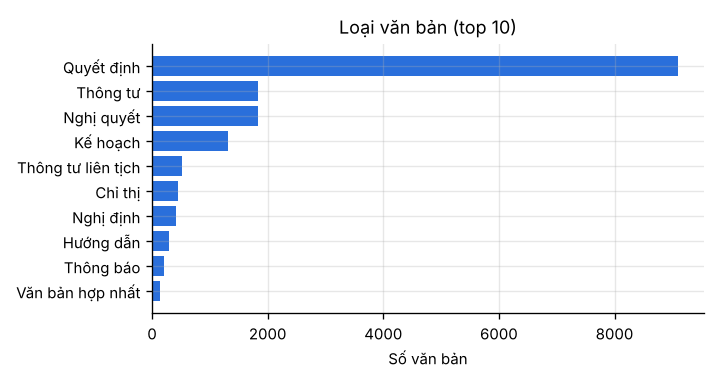
\includegraphics[width=\linewidth]{corpus_doc_types.png}\end{subfigure}
\begin{subfigure}{.49\linewidth}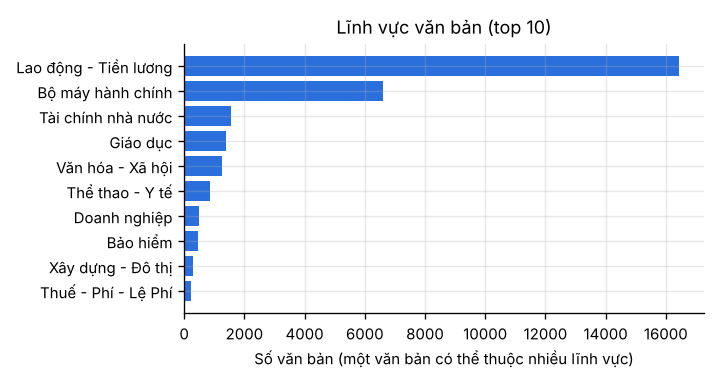
\includegraphics[width=\linewidth]{corpus_fields.png}\end{subfigure}
\caption{Loại văn bản và lĩnh vực trong corpus.}
\end{figure}

\subsection{Bộ câu hỏi RES}
\begin{itemize}
  \item 2.745 cặp hỏi--đáp. Câu hỏi trung bình 31 từ. Câu trả lời tham chiếu \textbf{trung bình 351 từ} (p95: 740 từ).
  \item 55\% câu trả lời mở đầu bằng ``Căn cứ\dots'' và 92\% có nhắc ``Điều N''. Đây là mẫu câu mà prompt cải tiến khai thác.
  \item 17\% câu hỏi ghi số hiệu văn bản ngay trong câu. 772 câu (28\%) không có số hiệu văn bản (``Không trích xuất được'').
  \item Văn bản được hỏi chủ yếu là của NHNN (ngân hàng, 1.256 câu) và Nghị định của Chính phủ (444 câu).
        Loại câu hỏi (phân loại bằng từ khóa): mô tả quy định (636), số liệu/thời hạn (464), có/không (329)\dots
\end{itemize}

\begin{figure}[H]
\centering
\begin{subfigure}{.52\linewidth}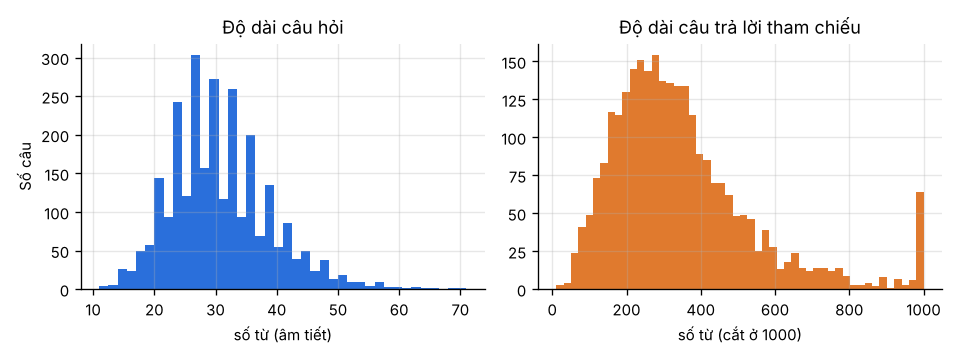
\includegraphics[width=\linewidth]{qa_lengths.png}\end{subfigure}
\begin{subfigure}{.46\linewidth}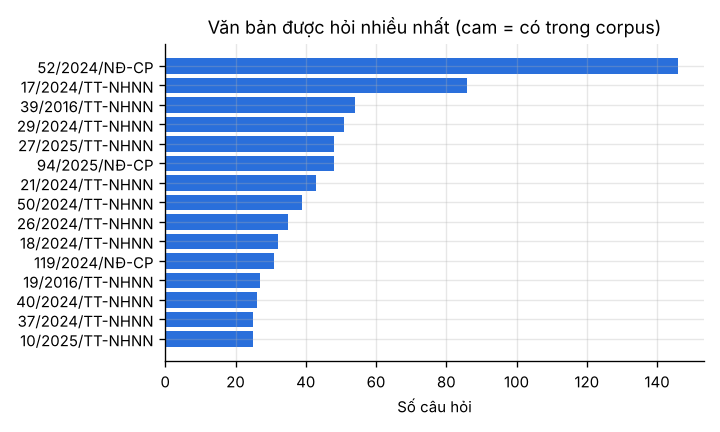
\includegraphics[width=\linewidth]{qa_top_refs.png}\end{subfigure}
\caption{Độ dài câu hỏi/câu trả lời và các văn bản được hỏi nhiều nhất (không có văn bản nào trong top 15 nằm trong corpus).}
\end{figure}

\subsection{Độ phủ: corpus và câu hỏi lệch nhau}
Chỉ \textbf{8/314} văn bản được hỏi có trong corpus, ứng với \textbf{51/2.745 câu (1{,}9\%)}.
Từ ``ngân hàng'' có trong 39\% câu hỏi nhưng chỉ ở 15\% văn bản, còn ``lao động'' có trong 0{,}9\% câu hỏi nhưng ở 98{,}5\% văn bản.
Văn bản được hỏi có trung vị năm 2024.

\begin{figure}[H]
\centering
\begin{subfigure}{.49\linewidth}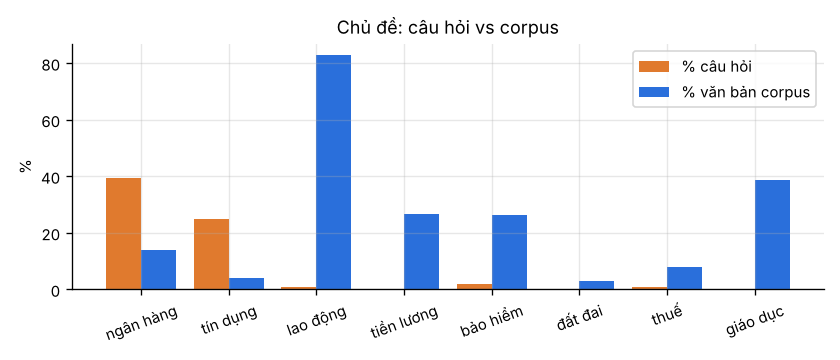
\includegraphics[width=\linewidth]{topic_mismatch.png}\end{subfigure}
\begin{subfigure}{.49\linewidth}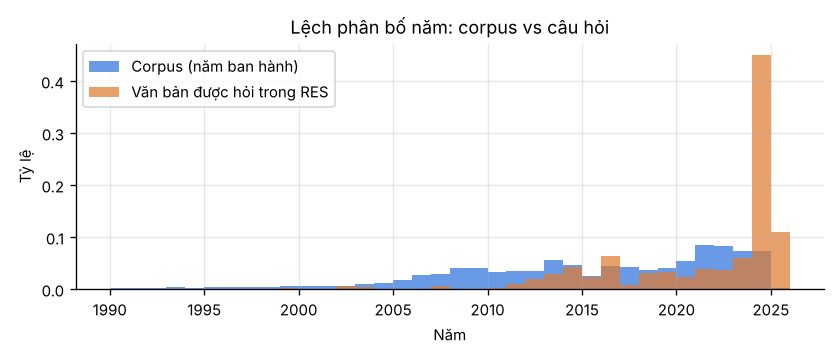
\includegraphics[width=\linewidth]{year_mismatch.png}\end{subfigure}
\caption{Chủ đề và năm ban hành: câu hỏi so với corpus.}
\end{figure}

\paragraph{Hệ quả cho thiết kế.}
(i) Với khoảng 98\% câu hỏi, retrieval chỉ có thể tìm văn bản liên quan về chủ đề, không thể tìm được văn bản nguồn.
Vì vậy tập đánh giá gồm \textbf{cả 51 câu có văn bản nguồn trong corpus (nhóm \emph{covered})} và 149 câu ngẫu nhiên (nhóm \emph{not\_covered}), và kết quả được báo cáo riêng từng nhóm.
(ii) Các chỉ số đo độ trùng từ với câu trả lời dài khoảng 350 từ, nên \emph{dạng} và \emph{độ dài} câu trả lời ảnh hưởng lớn tới điểm.
(iii) LLM phải được dặn không bịa số hiệu văn bản hay số Điều.

% =====================================================================
\section{Baseline}
Baseline: chunk 2.000/50 ký tự trên văn bản đã chuyển hết sang chữ thường $\rightarrow$ \path{keepitreal/vietnamese-sbert}~\cite{vietsbert,reimers2019sbert} $\rightarrow$ FAISS~\cite{johnson2021faiss} (L2), lấy top-5
$\rightarrow$ prompt 3 dòng $\rightarrow$ \path{Qwen/Qwen1.5-1.8B}~\cite{qwen15} (bản \emph{base}, chưa tinh chỉnh để làm theo chỉ dẫn), greedy, \texttt{max\_new\_tokens}=256.

\paragraph{Output của baseline có lẫn prompt.}
\texttt{HuggingFacePipeline.generate} của LangChain~\cite{langchain} mặc định \texttt{skip\_prompt=False}, còn Transformers~\cite{wolf2020transformers} mặc định \texttt{return\_full\_text=True}.
Em đã kiểm tra điều này trong mã nguồn \texttt{langchain\_huggingface}.
Vì vậy chuỗi được chấm điểm gồm cả prompt và 5 chunk ngữ cảnh: trung bình \textbf{2.369 từ}, so với 351 từ của câu tham chiếu.
Token Overlap đo tỷ lệ từ của câu tham chiếu xuất hiện trong output và không phạt độ dài, nên được lợi rất lớn (0{,}768).
Em báo cáo cả \emph{baseline} (giữ nguyên hành vi gốc, dùng làm mốc chính thức) và \emph{baseline\_noecho} (chỉ chấm phần mô hình sinh ra).
Notebook gốc chỉ chạy 30 câu; em chạy lại baseline trên đúng 200 câu của tập đánh giá.

% =====================================================================
\section{Phương pháp cải tiến}
\begin{table}[H]
\centering\small
\caption{So sánh từng thành phần của baseline và hệ thống cải tiến.}
\begin{tabularx}{\linewidth}{@{}l>{\raggedright}p{2.6cm}X@{}}
\toprule
& \textbf{Baseline} & \textbf{Cải tiến} \\
\midrule
Tiền xử lý & lowercase, \textbackslash n $\rightarrow$ space & chuẩn hóa NFC, nối dòng bị ngắt, \textbf{giữ hoa/thường}, tách metadata, bỏ MỤC LỤC/VĂN BẢN LIÊN QUAN \\
Chunking & ký tự 2.000/50 & \textbf{theo Chương/Điều}, 1.000/150, cắt ở biên câu/từ; gắn \textbf{header} (tên văn bản, số hiệu, Điều) vào mỗi chunk. Tổng 384.612 chunk \\
Retrieval & dense sbert & \textbf{BM25}~\cite{robertson2009bm25} (âm tiết + bigram) + dense \texttt{vietnamese-bi-encoder}~\cite{bkaibiencoder,duc2024vietrag} (nền PhoBERT~\cite{nguyen2020phobert}, tách từ bằng pyvi~\cite{pyvi}), ghép bằng \textbf{RRF}~\cite{cormack2009rrf}; ưu tiên văn bản có số hiệu ghi trong câu hỏi; tối đa 3 chunk mỗi văn bản \\
Reranking & -- & cross-encoder \texttt{bge-reranker-v2-m3}~\cite{bgereranker,chen2024m3}, lấy top-20 rồi giữ top-5 \\
LLM & Qwen1.5-1.8B (base) & \textbf{Qwen2.5-3B-Instruct}~\cite{qwen25}, dùng chat template, greedy, repetition penalty 1{,}05, tối đa 640 token \\
Prompt & 3 dòng chung chung & vai luật sư; mẫu \textbf{``Căn cứ tại Điều \dots\ quy định:''}; nguồn đánh số kèm header và tình trạng hiệu lực; cấm bịa số hiệu/Điều; nói rõ khi không tìm thấy \\
Few-shot & -- & 1 ví dụ hỏi--đáp cố định, chỉ lấy từ phần dữ liệu ngoài tập đánh giá \\
Hậu xử lý & -- & bỏ prompt bị lặp, token đặc biệt và câu lặp \\
\bottomrule
\end{tabularx}
\end{table}

\paragraph{Lý do lựa chọn.}
Chunk nhỏ, có header giúp mỗi đoạn tự đứng được (retriever và LLM đều biết đoạn thuộc văn bản nào, Điều nào), và cho phép đưa nhiều nguồn hơn vào context của model 3B.
Văn bản pháp luật có nhiều từ khóa chính xác (số hiệu, thuật ngữ) nên BM25 mạnh, còn dense bắt được câu diễn đạt khác đi; cross-encoder sắp xếp lại thứ hạng chính xác hơn.
BM25 được tự cài bằng ma trận thưa (scipy) kết hợp hashing, vì thư viện \texttt{bm25s} bị hết RAM khi giữ khoảng 180 triệu token dạng chuỗi.
Cuối cùng, câu trả lời tham chiếu dài và theo mẫu cố định, nên LLM instruct cùng prompt theo mẫu giúp câu trả lời đúng dạng và đủ dài.

% =====================================================================
\section{Thí nghiệm}
\paragraph{Thiết lập.}
200 cặp hỏi--đáp cố định (\file{data/eval_set.csv}, seed 42): 51 câu covered và 149 câu not\_covered.
Chạy trên Kaggle với GPU NVIDIA T4 miễn phí: khoảng 9--13 giây mỗi câu khi chạy theo lô, VRAM tối đa 4{,}5--7{,}4 GB.
Cosine luôn được tính bằng \path{keepitreal/vietnamese-sbert}, cùng embedding với baseline, để so sánh công bằng.
Các công thức metric giống hệt notebook baseline (có kiểm thử tự động).

\subsection{Retrieval}
\begin{table}[H]
\centering\small
\caption{Retrieval, chưa dùng LLM. DocRecall/MRR tính trên 51 câu covered. CtxTokenRecall là tỷ lệ từ của câu trả lời tham chiếu có mặt trong ngữ cảnh lấy về (tính trên cả 200 câu).}
\label{tab:retrieval}
\begin{tabular}{@{}lccccc@{}}
\toprule
Cấu hình ($k=5$) & DocRecall@1 & DocRecall@5 & MRR & CtxTokenRecall & Ký tự ngữ cảnh \\
\midrule
BM25, chunk baseline 2.000 & 0{,}471 & 0{,}784 & 0{,}606 & \best{0{,}753} & 9.739 \\
BM25, chunk theo Điều & 0{,}471 & 0{,}784 & 0{,}606 & 0{,}633 & 4.059 \\
Dense bi-encoder & 0{,}294 & 0{,}667 & 0{,}448 & 0{,}593 & 3.608 \\
Hybrid (RRF) & 0{,}471 & 0{,}843 & 0{,}622 & 0{,}653 & 3.841 \\
Hybrid + rerank & \best{0{,}608} & \best{0{,}863} & \best{0{,}727} & 0{,}655 & 3.960 \\
\bottomrule
\end{tabular}
\end{table}

\begin{figure}[H]
\centering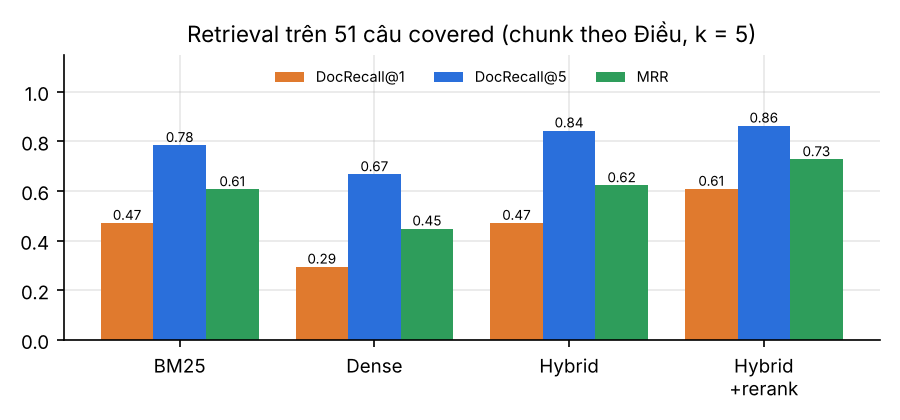
\includegraphics[width=.72\linewidth]{retrieval.png}
\caption{Kết hợp hai cách tìm kiếm và xếp hạng lại giúp văn bản nguồn lên đầu danh sách nhiều hơn.}
\end{figure}

Trên corpus này, dense đứng riêng kém hơn BM25. Kết hợp hai cách tăng DocRecall@5 từ 0{,}784 lên 0{,}843.
Reranker đưa văn bản đúng lên đầu nhiều hơn hẳn: DocRecall@1 từ 0{,}471 lên 0{,}608, MRR từ 0{,}606 lên 0{,}727.
CtxTokenRecall cao nhất ở chunk 2.000 chỉ vì ngữ cảnh dài gấp 2{,}5 lần. Khi lấy cùng khoảng 8k ký tự (chunk theo Điều, $k=10$), DocRecall đạt 0{,}824 so với 0{,}784.

\subsection{Kết quả chính và ablation}
\begin{table}[H]
\centering\small
\caption{Kết quả trên 200 câu, mỗi dòng thêm một thành phần. ($^{*}$) cao giả tạo vì output có lẫn khoảng 2.400 từ prompt và ngữ cảnh (mục 3). F được báo cáo riêng (mục 5.5).}
\label{tab:main}
\resizebox{\linewidth}{!}{%
\begin{tabular}{@{}lcccccr@{}}
\toprule
Cấu hình & Cosine & Jaccard & Token Overlap & BLEU & ROUGE-L & Số từ \\
\midrule
Baseline (gốc, output lẫn prompt) & 0{,}6991 & 0{,}2012 & \best{0{,}7675}$^{*}$ & 0{,}1173 & 0{,}0959 & 2.369 \\
Baseline\_noecho (chỉ phần sinh ra) & 0{,}5768 & 0{,}1510 & 0{,}1064 & 0{,}0426 & 0{,}1127 & 79 \\
\midrule
A: + Qwen2.5-3B-Instruct + prompt mới & 0{,}7259 & 0{,}2599 & 0{,}2946 & 0{,}2145 & 0{,}1999 & 208 \\
B: + chunk theo Điều + BM25 & 0{,}7316 & 0{,}2882 & 0{,}3382 & 0{,}2530 & 0{,}2257 & 235 \\
C: + hybrid (BM25 + dense) & 0{,}7363 & 0{,}2974 & 0{,}3483 & 0{,}2589 & 0{,}2293 & 237 \\
D: + rerank & 0{,}7517 & \best{0{,}3120} & 0{,}3692 & \best{0{,}2784} & 0{,}2424 & 248 \\
\textbf{E: + 1 ví dụ few-shot (hệ thống cuối)} & \best{0{,}7636} & 0{,}3063 & 0{,}3692 & 0{,}2740 & \best{0{,}2463} & 235 \\
\midrule
\emph{F: E + hỏi--đáp tương tự làm tham khảo} & \emph{0{,}7676} & \emph{0{,}3692} & \emph{0{,}4187} & \emph{0{,}3276} & \emph{0{,}3099} & \emph{242} \\
\bottomrule
\end{tabular}}
\end{table}

\begin{figure}[H]
\centering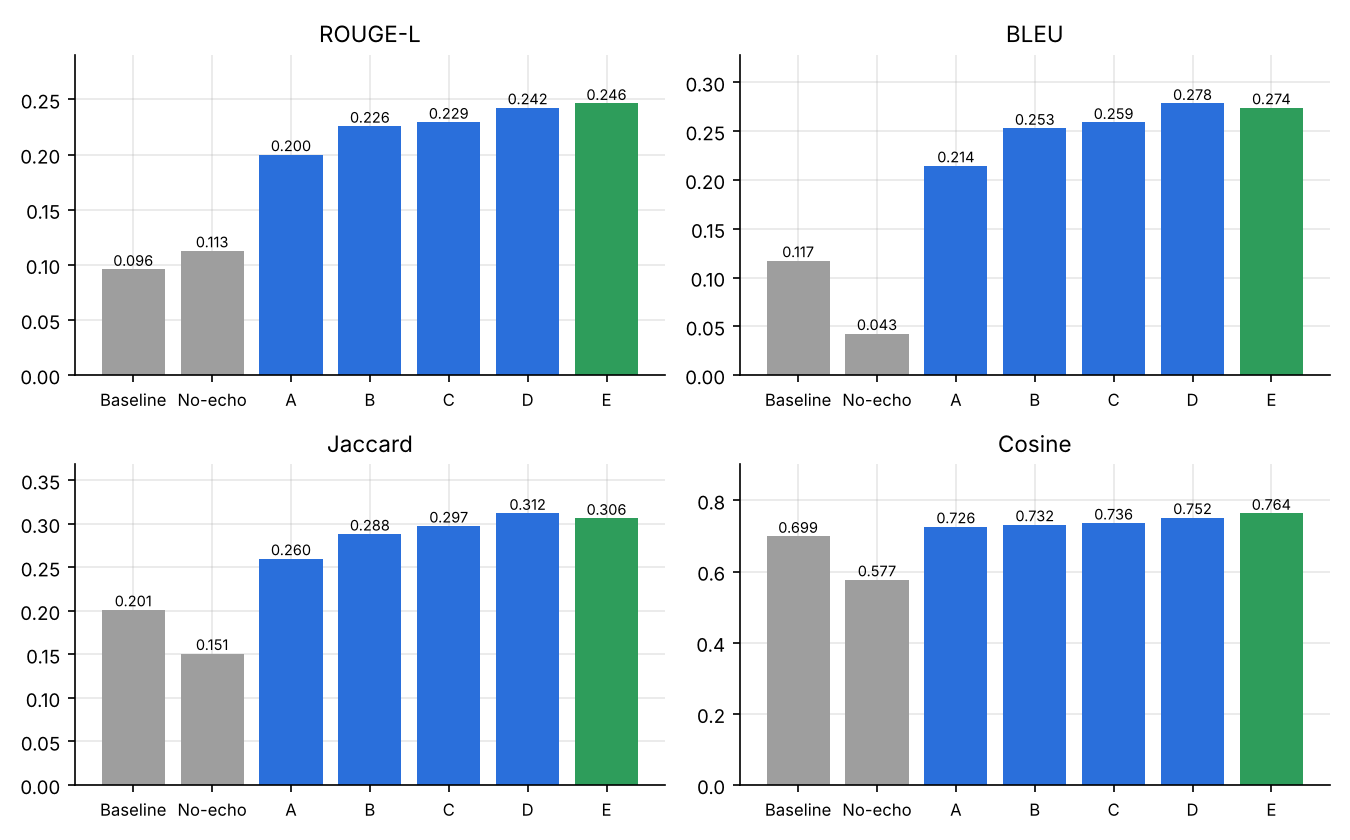
\includegraphics[width=.9\linewidth]{ablation_metrics.png}
\caption{Bốn chỉ số qua từng bước. Màu xám là baseline, màu xanh dương là các bước trung gian, màu xanh lá là hệ thống cuối E.}
\end{figure}

\begin{table}[H]
\centering\small
\caption{Mức cải thiện của hệ thống cuối. BLEU (đo precision, có brevity penalty) và ROUGE-L (F1) không bị ảnh hưởng bởi việc lẫn prompt như Token Overlap.}
\resizebox{\linewidth}{!}{%
\begin{tabular}{@{}lccccc@{}}
\toprule
E so với & Cosine & Jaccard & Token Overlap & BLEU & ROUGE-L \\
\midrule
Baseline (gốc) & +0{,}065 (+9\%) & +0{,}105 (+52\%) & $-0{,}398^{*}$ & +0{,}157 (+134\%) & +0{,}150 (+157\%) \\
Baseline\_noecho & +0{,}187 (+32\%) & +0{,}155 (+103\%) & +0{,}263 (+247\%) & +0{,}231 (+543\%) & +0{,}134 (+119\%) \\
\bottomrule
\end{tabular}}
\end{table}

\subsection{Phân tích theo nhóm câu hỏi}
\begin{figure}[H]
\centering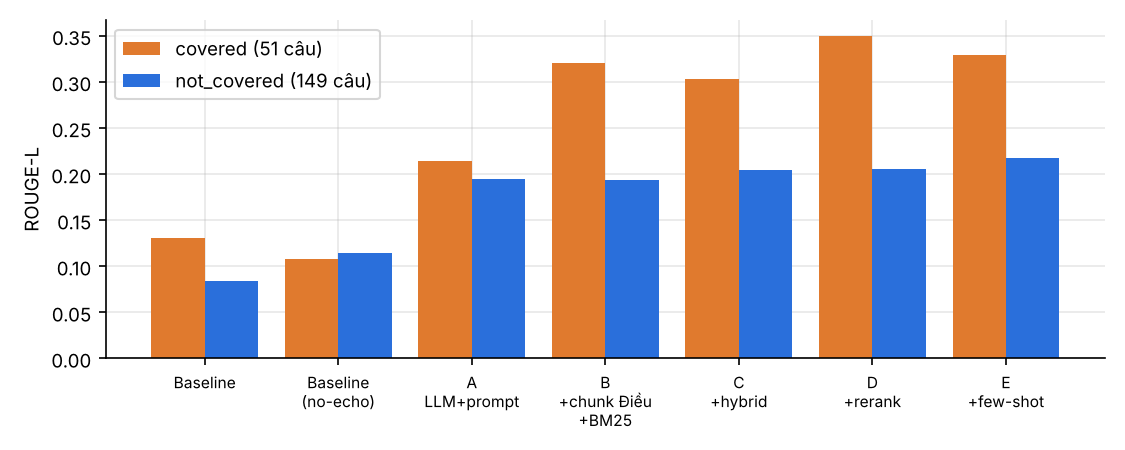
\includegraphics[width=.8\linewidth]{rouge_by_group.png}
\caption{ROUGE-L theo nhóm. Retrieval tốt hơn (từ B trở đi) chủ yếu giúp nhóm covered.}
\end{figure}

\begin{itemize}
  \item \textbf{A (đổi LLM và prompt)} mang lại bước nhảy lớn nhất: ROUGE-L từ 0{,}096 lên 0{,}200, BLEU tăng gấp đôi, dù retrieval vẫn như baseline.
        Model instruct trả lời đúng trọng tâm, đủ dài và theo mẫu: 66--88\% câu mở đầu bằng ``Căn cứ\dots'', còn baseline là 0\%.
  \item \textbf{B (chunk theo Điều + BM25)} tăng mạnh ở nhóm covered (ROUGE-L từ 0{,}215 lên 0{,}320) nhưng gần như không đổi ở not\_covered (0{,}195 xuống 0{,}193).
        Đúng như dự đoán: retrieval tốt hơn chỉ giúp khi văn bản nguồn có trong corpus.
  \item \textbf{C (hybrid)} cải thiện nhẹ. \textbf{D (rerank)} cho điểm covered cao nhất (ROUGE-L 0{,}350, Cosine 0{,}843).
  \item \textbf{E (few-shot)} cho Cosine và ROUGE-L tổng cao nhất, tốt nhất ở nhóm not\_covered (ROUGE-L 0{,}218), và ít bịa số hiệu nhất (mục 5.4).
        Vì vậy E được chọn làm hệ thống cuối; D là phương án thay thế gần tương đương.
\end{itemize}

\subsection{Phân tích lỗi}
\begin{table}[H]
\centering\small
\caption{``Bịa số hiệu'': câu trả lời nhắc một số hiệu văn bản không xuất hiện ở đâu trong ngữ cảnh lấy về.}
\begin{tabular}{@{}lccc@{}}
\toprule
Cấu hình & Bịa số hiệu (covered / not\_cov.) & Nói ``không tìm thấy'' & Mở đầu ``Căn cứ\dots'' \\
\midrule
Baseline\_noecho & 4\% / 9\% & 2\% / 7\% & 0\% / 0\% \\
A & 31\% / 35\% & 18\% / 39\% & 88\% / 66\% \\
D & 6\% / 17\% & 6\% / 11\% & 100\% / 97\% \\
E & \best{2\% / 11\%} & 16\% / 17\% & 77\% / 66\% \\
\bottomrule
\end{tabular}
\end{table}

\begin{itemize}
  \item Ở cấu hình A, ngữ cảnh thường không liên quan, nên model ``căn cứ'' vào văn bản nó tự nhớ hoặc tự bịa (31--35\%).
        Khi retrieval tốt hơn (D, E), tỷ lệ này giảm còn 2--17\%.
  \item \textbf{Ví dụ tốt (covered):} câu hỏi về lịch nghỉ 30/4/2025. Hệ thống lấy đúng Thông báo 6150/TB-BLĐTBXH, trích đúng đợt nghỉ 5 ngày từ 30/4 đến 04/5/2025.
        Tuy vậy, model diễn giải sai ngày làm bù: văn bản quy định làm bù vào thứ Bảy 26/4, còn model coi 03/5 và 04/5 là ngày làm bù. Đây là hạn chế về suy luận của model 3B.
  \item \textbf{Ví dụ điển hình của nhóm not\_covered:} câu hỏi về quyền và nghĩa vụ của đối tượng thanh tra ngân hàng (đáp án ở Điều 208 Luật Các tổ chức tín dụng 2024, không có trong corpus).
        Hệ thống lấy về Nghị định 88/2016/NĐ-CP về \emph{ngân hàng giám sát} quỹ hưu trí và trả lời dựa trên văn bản này.
        Câu trả lời bám đúng ngữ cảnh nhưng sai văn bản, hệ quả trực tiếp của việc corpus thiếu văn bản ngân hàng.
  \item \textbf{Baseline} thường chỉ lặp lại câu hỏi và để lộ token ``assistant'', vì Qwen1.5-1.8B bản base không làm theo chỉ dẫn.
\end{itemize}

\subsection{Ablation phụ F: dùng bộ hỏi--đáp làm tài liệu tham khảo}
Cấu hình F thêm vào prompt 2 cặp hỏi--đáp tương tự nhất, lấy từ 2.545 cặp \emph{không thuộc} tập đánh giá; các câu gần như trùng lặp (Jaccard $>0{,}8$) bị loại.
ROUGE-L tăng từ 0{,}246 lên 0{,}310, gần như hoàn toàn ở nhóm not\_covered (0{,}218 lên 0{,}310).
Tuy nhiên đây là tận dụng dữ liệu hỏi--đáp chứ không phải RAG trên corpus, và câu trả lời thường chép số hiệu văn bản từ các cặp đó (35\% ở not\_covered).
Vì vậy em \textbf{không} dùng F làm kết quả chính. F chỉ cho thấy nếu corpus có đúng văn bản ngân hàng thì hệ thống có thể đạt mức nào.

% =====================================================================
\section{Demo}
Demo chạy trên Kaggle (GPU T4 miễn phí). Notebook dùng khi quay video, có sẵn output, là \file{notebooks/demo_chatbox.ipynb}
(bản sinh từ script: \file{notebooks/demo.ipynb}). Người dùng nhập câu hỏi vào ô hỏi ngay trong notebook,
hệ thống trả về câu trả lời kèm danh sách nguồn (tên văn bản, Điều, tên file, đoạn trích), mỗi câu khoảng 20--60 giây.
Ngoài ra có thể chạy bằng dòng lệnh (\file{app/demo.py --cli}) hoặc giao diện Gradio.
Các câu hỏi mẫu được chọn trong lĩnh vực mà corpus có và đã kiểm tra là tìm đúng văn bản:
lương cơ sở từ 01/7/2024 (Nghị định 73/2024/NĐ-CP), nghỉ hằng năm (Bộ luật Lao động 2019, Điều 113),
trợ cấp thôi việc (Nghị định 145/2020/NĐ-CP), lịch nghỉ 30/4 năm 2025 (Thông báo 6150/TB-BLĐTBXH).
Video demo: \url{\videolink}.

% =====================================================================
\section{Hạn chế và hướng phát triển}
\begin{itemize}
  \item \textbf{Corpus và câu hỏi lệch nhau:} chỉ khoảng 2\% câu hỏi có văn bản nguồn trong corpus.
        Ở nhóm not\_covered, phần điểm tăng chủ yếu đến từ việc câu trả lời đúng \emph{dạng} hơn, chứ không đúng \emph{nội dung} hơn.
  \item Các metric đo độ trùng từ nên ưu tiên câu trả lời dài và theo mẫu; chúng không đo được tính đúng đắn pháp lý.
  \item Model 3B đôi khi suy luận sai chi tiết (ngày, số liệu) dù đã lấy đúng văn bản.
  \item Chỉ đánh giá 200/2.745 câu do giới hạn GPU miễn phí. Tập đánh giá cố ý chứa toàn bộ 51 câu covered, nên kết quả được báo cáo riêng từng nhóm.
  \item \textbf{Hướng phát triển:} bổ sung văn bản ngân hàng (NHNN) và các văn bản năm 2024--2025 vào corpus;
        lọc theo tình trạng hiệu lực; thử LLM lớn hơn trong giới hạn 4B hoặc tinh chỉnh (fine-tune) trên phần hỏi--đáp ngoài tập đánh giá.
\end{itemize}

% =====================================================================
\section{Kết luận}
Trên cùng 200 câu, hệ thống cải tiến vượt baseline gốc ở Cosine (+9\%), Jaccard (+52\%), BLEU (+134\%) và ROUGE-L (+157\%).
So với baseline đã bỏ phần prompt lẫn vào, nó tốt hơn ở cả 5 chỉ số.
Phần lớn mức tăng đến từ việc đổi sang LLM instruct và thiết kế prompt theo mẫu câu trả lời pháp lý.
Retrieval tốt hơn (chunk theo Điều, hybrid, rerank) tăng thêm mạnh ở những câu có văn bản nguồn trong corpus
(ROUGE-L từ 0{,}215 lên 0{,}329--0{,}350) và giảm rõ việc bịa số hiệu văn bản (từ 31--35\% xuống 2--11\%).

% =====================================================================
\phantomsection\addcontentsline{toc}{section}{Tài liệu tham khảo}
\bibliographystyle{IEEEtran}
\bibliography{references}


% =====================================================================
\appendix
\section{Mã nguồn, dữ liệu và hướng dẫn chạy lại}\label{app:manual}
Toàn bộ bài nộp nằm trong repo \url{\githublink}. Bản đầy đủ của phụ lục này là \file{README.md} trong repo.

\subsection{Thành phần bài nộp}
\begin{center}\small
\begin{tabularx}{\linewidth}{@{}lX@{}}
\toprule
Thành phần & Vị trí trong repo \\
\midrule
Mã nguồn & \file{src/} (thư viện), \file{scripts/} (các bước chạy), \file{app/} (demo), \file{notebooks/} (Kaggle), \file{tests/} \\
Dữ liệu & \file{Dataset/export_1/}: 16.439 văn bản .txt, khoảng 442MB; \file{doc/RES.xlsx}: 2.745 cặp QA.
           Cả hai đã nằm trong git, không phải tải riêng. \file{data/eval_set.csv}: 200 câu đánh giá cố định (seed 42) \\
Hướng dẫn & \file{README.md} (cài đặt, chạy lại, demo, kết quả mong đợi) \\
Kết quả & \file{results/predictions/}: câu trả lời từng câu của mọi cấu hình; \file{results/metrics/}; \file{results/eda/} \\
\bottomrule
\end{tabularx}
\end{center}

\subsection{Cài đặt}
\begin{verbatim}
git clone -b RAG-based-chatbot-system \
    https://github.com/dinhthithuthuyduphong-bot/LAB.git
cd LAB
pip install -r requirements.txt        # hoặc requirements-lock.txt
pip install -r requirements-gpu.txt    # chỉ khi có GPU
\end{verbatim}

\subsection{Kiểm tra nhanh, không cần GPU (khoảng 10 phút)}
Thầy có thể kiểm tra lại kết quả chỉ bằng CPU theo ba bước sau.
\begin{enumerate}
  \item \textbf{Tính lại metric} từ câu trả lời đã lưu: \verb|python -I scripts/evaluate.py --no-cosine|.
        Bốn metric từ vựng phải trùng với Bảng~\ref{tab:main}. Nếu lệnh \verb|git diff results/metrics/summary.csv| không in ra gì thì kết quả đã khớp.
  \item \textbf{Dựng lại dữ liệu và chỉ mục BM25} (khoảng 5 phút):
\begin{verbatim}
python -I scripts/build_corpus.py         # 16439 documents
python -I scripts/prepare_data.py --n 200 # 200 câu: 51 covered + 149
python -I scripts/eda.py
python -I scripts/build_chunks.py --strategy legal     # 384,612 chunks
python -I scripts/build_chunks.py --strategy baseline
python -I scripts/build_bm25.py --chunks legal
python -I scripts/build_bm25.py --chunks baseline
python -I scripts/eval_retrieval.py --k 5
python -I tests/test_core.py
\end{verbatim}
  \item \textbf{Demo không cần GPU} (chỉ hiện các đoạn văn bản tìm được):
\begin{verbatim}
python -I app/demo.py --llm extractive \
    --cli "Mức lương cơ sở từ 01/7/2024 là bao nhiêu?"
\end{verbatim}
\end{enumerate}
Em đã chạy lại đúng các bước trên từ một bản clone sạch (Linux, Python 3.13, RAM 16GB).
Mọi bước đều chạy được, và \file{data/}, \file{results/eda/}, \file{results/metrics/} sinh ra khớp với bản đã nộp.

\subsection{Chạy lại toàn bộ có GPU}
Mở \file{notebooks/run_on_kaggle.ipynb} trên Kaggle, bật GPU T4 và Internet, rồi chọn \emph{Save \& Run All (Commit)}.
Notebook tự clone repo, tạo index FAISS, chạy baseline và các cấu hình A--F, rồi tính đủ 5 metric.
Mỗi cấu hình mất khoảng 30--45 phút cho 200 câu.
Câu trả lời được lưu dần vào \file{results/predictions/}, nên nếu phiên bị ngắt thì chạy lại sẽ tiếp tục từ chỗ dừng.
Sau đó chạy \file{scripts/error_analysis.py}, \file{make_tables.py} và \file{make_report_figures.py} trên CPU để sinh bảng và hình cho báo cáo.
Muốn chạy thử nhánh GPU mà không tốn quota, dùng \file{tests/smoke_gpu_path.py}: script này dùng model tí hon tạo ngay trên máy và chạy được trên CPU.

\end{document}
